\documentclass[12pt,a4paper,final]{article}
\usepackage[utf8]{inputenc}
\usepackage{amsmath}
\usepackage{amsfonts}
\usepackage{amssymb}
\usepackage{graphicx}
\usepackage{enumitem}
\usepackage{amsmath}
\usepackage[portuguese]{babel}
\usepackage[utf8]{inputenc}
\usepackage{pdfpages}
\usepackage[portuguese]{babel}
\usepackage[T1]{fontenc}
\usepackage{amsmath}
\usepackage{amsfonts}
\usepackage{amssymb}
\usepackage{graphicx}
\usepackage[left=2.5cm,right=2.5cm,top=2.5cm,bottom=2.5cm]{geometry}
\author{Gerente: Luan Bodner do Rosário}
\title{Plano de Projeto - Projeto 1}
\title{Laudo PBR refente ao projeto II }

\begin{document}

      	\begin{titlepage}
       	\LARGE
       	\begin{center}
       	\vspace{5cm} 
       	\textbf{Universidade Tecnológica Federal do Paraná \\ \vspace{1.8cm}}
       	
\includegraphics[scale=0.35]{logoutfpr.jpg} \\ \vspace{1.8cm}
       	\textit{Engenharia de Software II} \vspace{2cm} \\
       	Luan Bodner do Rosário \\ 1509950 \vspace{2cm} \\ 
       	PROJETO 1 - PLANEJAMENTO DE DESENVOLVIMENTO DE SOFTWARE \vspace{2cm} \\
      	Departamento de Ciência da Computação (DACOM) 
       	
   	\end{center}
    \end{titlepage}	

\tableofcontents
\newpage
\section{Planejamento}

Este documento tem o intuíto de definir e dividir as principais tarefas do sistema a ser implementado para a disciplina de Engenharia de Software 2.\\
Para a definição das tarefas será utilizado o método EAP(Estrutura Analítica do Projeto) e com base nessa divisão, será utilizado o PERT(\textit{Program Evaluation and Review Technique}) para fazer a estimativa de tempo de cada uma dessas partes do sistema.
A EAP do projeto é definida conforme:

\begin{enumerate}
\item \textbf{Hemosystem}
\begin{enumerate}[label*=\arabic*.]
\item \textbf{Documentação}
\begin{enumerate}[label*=\arabic*.]
\item \textit{Perspective Base Reading}
\item Atualização do Documento de Requisitos
\item Diagramas de Caso de Uso
\item Diagramas de Classe
\item Revisão dos Documentos
\end{enumerate}
\item \textbf{Desenvolvimento}
\begin{enumerate}[label*=\arabic*.]
\item Criação das classes base
\item Definição do BD
\item Revisão do BD
\item Implementação das funcionalidades definidas pelo usuário
\item Implementação da Interface entre as classes
\item Definição das \textit{views} do BD
\end{enumerate}
\item \textbf{Interface}
\begin{enumerate}[label*=\arabic*.]
\item Definição das telas
\item Conectar a interface com as funcionalidades
\end{enumerate}
\item \textbf{Testes}

\end{enumerate}
\end{enumerate}


\newpage
As tarefas a serem implementadas prévia às tarefas de programação são:

\begin{enumerate}
\item Documentação do Projeto
\begin{enumerate}

\item Perspective Base Reading : Tarefa já concluida e documentada no laudo presente no repositório do Projeto.

\item Atualização do Documento de Requisitos: Tarefa já concluida e documentada no laudo presente no repositório do Projeto.

\item Diagrama de Classe : Tarefa que ainda deverá ser realizada pelo Projetista Josimar Loch para que possa ser levado para revisão e refinamento.
\begin{itemize}
\item Estimativa de tempo para término da tarefa : \\
Dada pela Fórmula : TE = O + 4 M + P / 6\\
Tempo Otimista (O) = 2.5h\\
Tempo Mais Provável (M) = 3.5h\\
Tempo Pessimista (P) = 5h\\
Tempo Esperado Total = 3.5h
\end{itemize} 

\item Diagrama de Caso de Uso : Também sob a responsabilidade do Projetista do projeto.
\begin{itemize}
\item Estimativa de tempo para término da tarefa : 
Tempo Otimista (O) = 2h\\
Tempo Mais Provável (M) = 3h\\
Tempo Pessimista (P) = 4h\\
Tempo Esperado Total = 3h
\end{itemize} 

\item Controle de Qualidade : Após a realização da primeira fase da criação de diagramas, ou mesmo concorrentemente com a sua realização, os diagramas devem ser analisados e refinados para que o processo de programação ocorra o mais rápido possível. Controle de qualidade será uma tarefa conjunta entre todos os membros da equipe.
\begin{itemize}
\item Estimativa de tempo para término da tarefa :\\
Tempo Otimista (O) = 1h\\
Tempo Mais Provável (M) = 2h\\
Tempo Pessimista (P) = 3h\\
Tempo Esperado Total = 2.5h
\end{itemize} 

\item Revisão : Após a revisão ser concluída e os erros listados previamente na análise PBR e encontrados na documentação forem encontrados, a documentação deverá passar por mudanças e submetidos em forma final. Responsabilidade do Projetista Josimar.
\begin{itemize}
\item Estimativa de tempo para término da tarefa :
Tempo Otimista (O) = 0.5h\\
Tempo Mais Provável (M) = 1h\\
Tempo Pessimista (P) = 3h\\
Tempo Esperado Total = 1.25h
\end{itemize} 
\end{enumerate}

Esses diagramas devem estar em um formato acessível para que o Programador Felipe Veiga Ramos possa lê-los com mais facilidade.\\
Todas essas sub-etapas podem (e devem) ser feitas concorrentemente.\\
As ferramentas utilizadas nessa parte do desenvolvimento são:
\begin{enumerate}
\item Astah
\item Github
\item Issue Tracker/Github
\end{enumerate}

\item Infraestrutura
\begin{enumerate}
\item Criação do Banco de Dados : Após a realização dos diagramas, o banco de dados deve ser criado com base nos dados necessários. Isso será uma tarefa conjunta entre o Projetista e o Programador.
Tempo Otimista (O) = 0.5h\\
Tempo Mais Provável (M) = 0.6h\\
Tempo Pessimista (P) = 0.7h\\
Tempo Esperado Total = 0.6h

\item Revisão/Testes de conexão BD : O banco deve ser revisado pelo Gerente do Projeto para evitar erros.
Tempo Otimista (O) = 1h\\
Tempo Mais Provável (M) = 1.5h\\
Tempo Pessimista (P) = 2h\\
Tempo Esperado Total = 1.5h
\end{enumerate}

As ferramentas utilizadas nessa parte do projeto está sujeito a escolha do Programador e Projetista.

\item Desenvolvimento
\begin{enumerate}

\item Criação das Classes Base : Criação das estruturas básicas e classes básicas para as operações lógicas do sistema a ser implementado. Todas as tarefas do desenvolvimento é tarega do Programador.
Tempo Otimista (O) = 2h\\
Tempo Mais Provável (M) = 3h\\
Tempo Pessimista (P) = 4h\\
Tempo Esperado Total = 3h

\item Implementação das funcionalidades : Com base nos diagramas e casos de uso definidos no documento original do projeto e o documento revisado com informações novas, as funcionalidades devem ser implementadas.
Tempo Otimista (O) = 12h\\
Tempo Mais Provável (M) = 15h\\
Tempo Pessimista (P) = 20h\\
Tempo Esperado Total = 40h

\item Implementação da interface entre as classes : Após as partes singulares do sistema estiverem implementadas, as partes do sistema devem ser conectadas de acordo com as especificações feitas.
Tempo Otimista (O) = 5h\\
Tempo Mais Provável (M) = 6h\\
Tempo Pessimista (P) = 8h\\
Tempo Esperado Total = 10h

\item Definição das \textit{views} do BD : Por questões de segurança, deve-se criar views diferentes no banco para cada nível de prioridade dos usuários.
Tempo Otimista (O) = 4h\\
Tempo Mais Provável (M) = 6h\\
Tempo Pessimista (P) = 8h\\
Tempo Esperado Total = 9h
\end{enumerate}

\item Interface
\begin{enumerate}
\item Definição das telas : Após o programa estiver completado, a interface com o usuário deve ser definida.
Tempo Otimista (O) = 3h\\
Tempo Mais Provável (M) = 4h\\
Tempo Pessimista (P) = 5h\\
Tempo Esperado Total = 5.5h
\item Conectar a interface com as funcionalidades : Após a interface estiver "desenhada", os módulos resultantes devem ser conectados ao código do programa e suas entradas/saídas.
Tempo Otimista (O) = 4h\\
Tempo Mais Provável (M) = 6h\\
Tempo Pessimista (P) = 8h\\
Tempo Esperado Total = 8h
\end{enumerate}

\item Testes : Com o programa completo, ou mesmo durante o seu desenvolvimento, o Testador Paulo Batista deve fazer os testes básicos definidos no PBR para verificar se o programa está funcionando corretamente.
Tempo Otimista (O) = 4h\\
Tempo Mais Provável (M) = 7h\\
Tempo Pessimista (P) = 8h\\
Tempo Esperado Total = 8h

\end{enumerate}

\section{Tabela de Atividades e Precedência}
\begin{center}
\begin{tabular}{|c|c|c|c|}
\hline 
Atividade & Descrição & Atividades Prec. & Duração \\ 
\hline 
A & Diagramas de Caso de Uso & - & 3h \\ 
\hline 
B & Diagramas de Classe & A & 3.5h \\ 
\hline 
C & Controle de Qualidade & B & 2.5h \\ 
\hline 
D & Revisão dos Documentos & C & 1.25h \\
\hline 
E & Criação das Classes básicas & C & 3h \\
\hline 
F & Criação do Banco & D & 0.6h \\ 
\hline 
G & Definir os campos & & \\ & das tabelas & F & 2h \\ 
\hline 
H & Criar métodos para & & \\ & lidar com o banco & F & 10h \\
\hline 
I & Criar métodos para & & \\ & interligar os & & \\ & módulos do sistema & O & 11h \\
\hline 
J & Definir métodos & & \\ & para registro dos doadores & E & 2.5h \\ 
\hline 
K & Definir métodos & & \\ & para registro dos exames & E &  3.5h \\ 
\hline 
L & Definir métodos para verificar & & \\ & a segurança quanto & & \\ & às bolsas de sangue & E & 3h \\ 
\hline 
M & Definir as pesquisas  & & \\ & possíveis dentro do banco & G,H,R & 10h \\ 
\hline 
N & Criar Interface para & & \\ & os usuários & K,J,L & 5h \\ 
\hline 
O & Conectar a interface com & & \\ & a aplicação e o banco de dados & N & 5h \\ 
\hline 
P & Testar funcinalidade dos métodos & I & 3h \\ 
\hline 
Q & Testar as entradas da interface & I & 5h \\ 
\hline 
R & Testar a conexão com & & \\ & o Banco de dados & F & 1.5h \\ 
\hline 
\end{tabular} 
\end{center}
A partir desta tabela de atividades, é possível contrurir o grafo que mostra o caminho crítico do projeto e auxilia no planejamento do projeto.\\
O grafo que representa as tarefas desta tabela foi contruido por meiro da linguagem .DOT. Ela é mostrada na imagem a seguir.
\subsection{Rede de atividades}
\begin{figure}\centering{
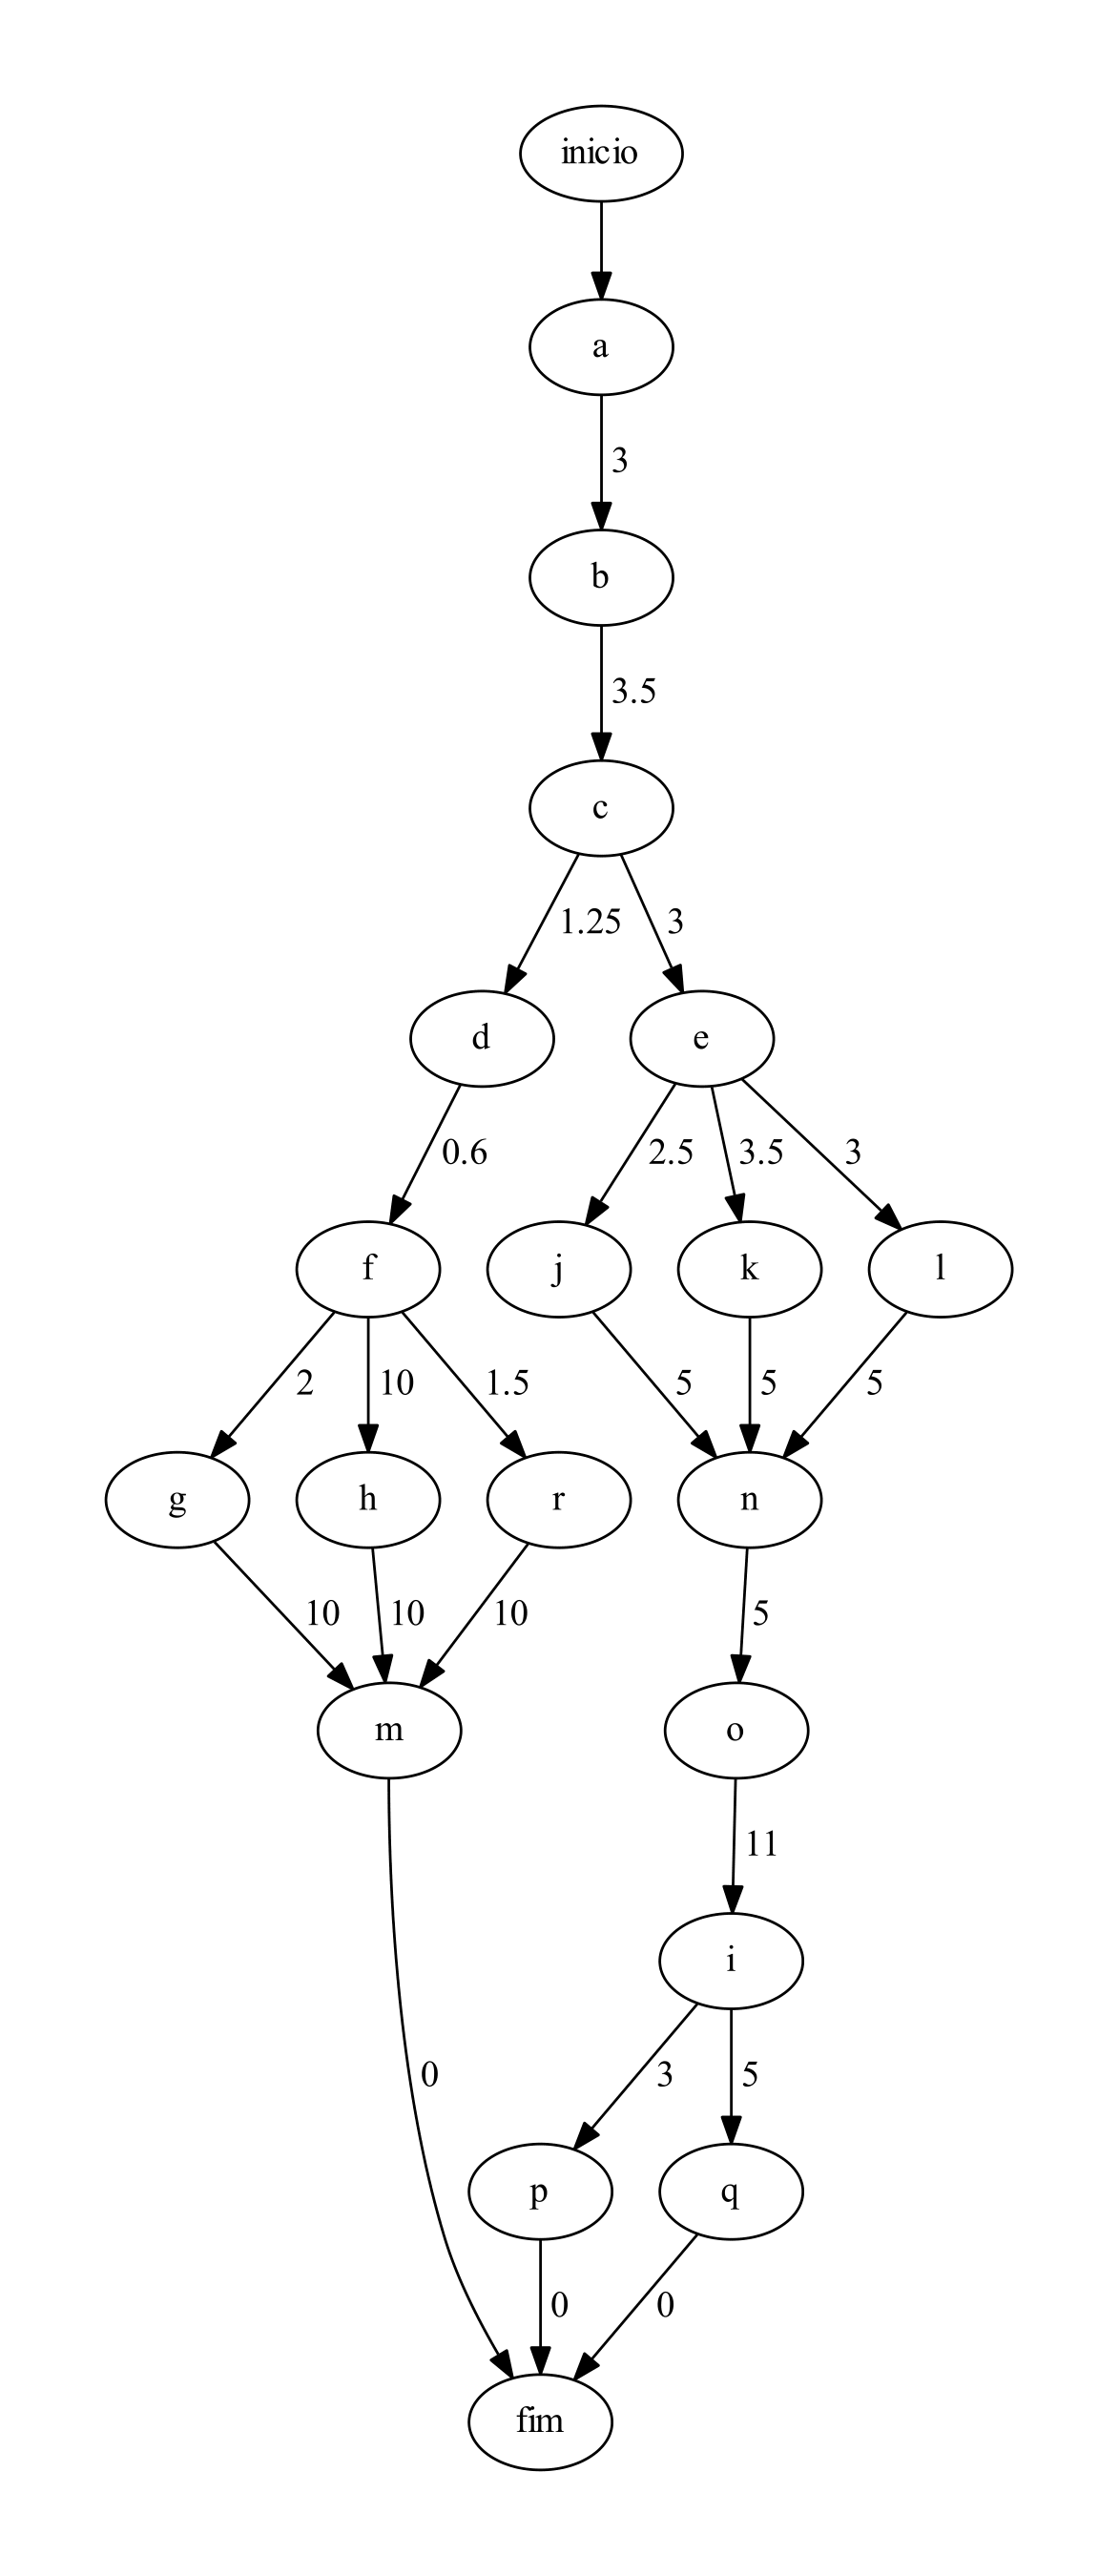
\includegraphics[scale=0.27]{Graph1.png}
\caption{Rede de atividades}}
\end{figure}
Por meio desta rede, podemos fazer o cálculo do caminho crítico, que é uma soma simples do maior caminho possível até que se chegue no final do projeto. Verificamos então que o caminho crítico é dado pela imagem a seguir:
\begin{figure}\centering{
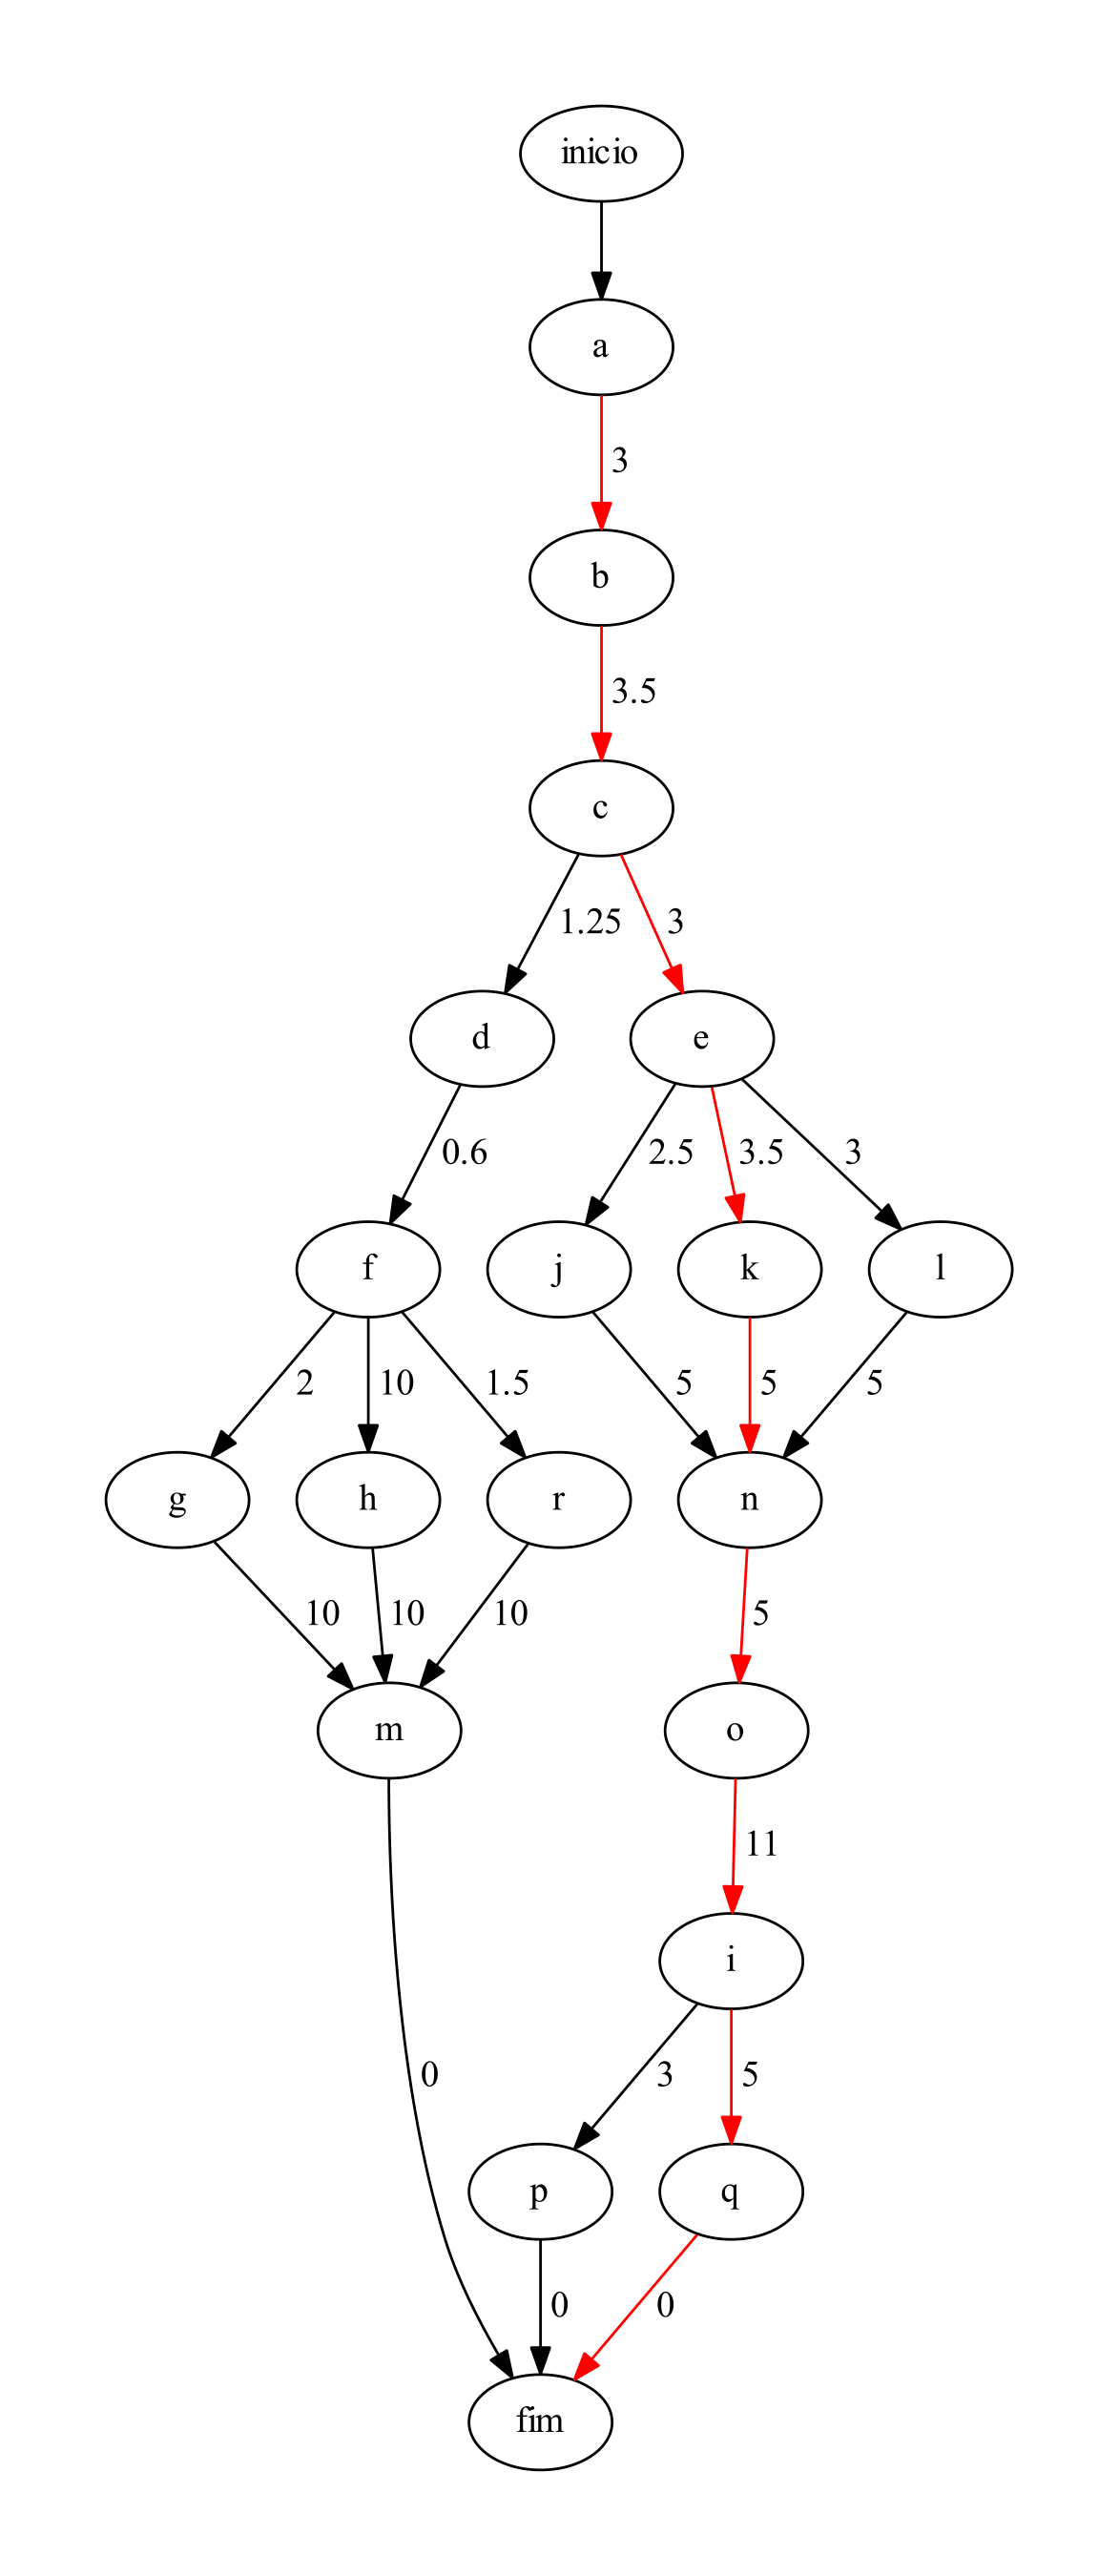
\includegraphics[scale=0.25]{CPGraph1.png}
\caption{Caminho Crítico}}
\end{figure}

Como planejado, foram montadas as redes de caminho para "cedo", de acordo com a fórmula :
\begin{equation}
Cedo = max(Cedo anterior + duração)
\end{equation}
E também para o caminho de tempo "tarde", de acordo com a fórmula:
\begin{equation}
Tarde = min(Tarde posterior - duração)
\end{equation}

Portanto, a rede e os pesos das arestas do grafo "cedo" na figura 3 e para o grafo "tarde" na figura 4.
Assim, por meio dos cálculos necessários, verificamos que a somatória dos caminhos críticos são semelhantes para cedo e tarde, que coloca o projeto dentro dos padrões, não sendo necessário fazer nenhum ajustamento quanto ao tempo de cada uma das tarefas listadas listadas.

\section{Horários de Trabalho}
Primeira Seção:
\begin{itemize}
\item Início : 6:30 da manhã, 24/05
\item Término : 11:00 da manhã, 24/05
\end{itemize}
Segunda Seção:
\begin{itemize}
\item Início : 9:00 da manhã, 14/06
\item Término : 11:00 da manhã 14/06
\end{itemize}
Terceira Seção:
\begin{itemize}
\item Início : 14:00 da tarde, 14/06
\item Término : 15:00 da tarde. 14/06
\end{itemize}
Quarta Seção:
\begin{itemize}
\item Início : 10:00 da tarde, 15/06
\item Término : 13:00 da tarde. 15/06
\end{itemize}

\begin{figure}\centering{
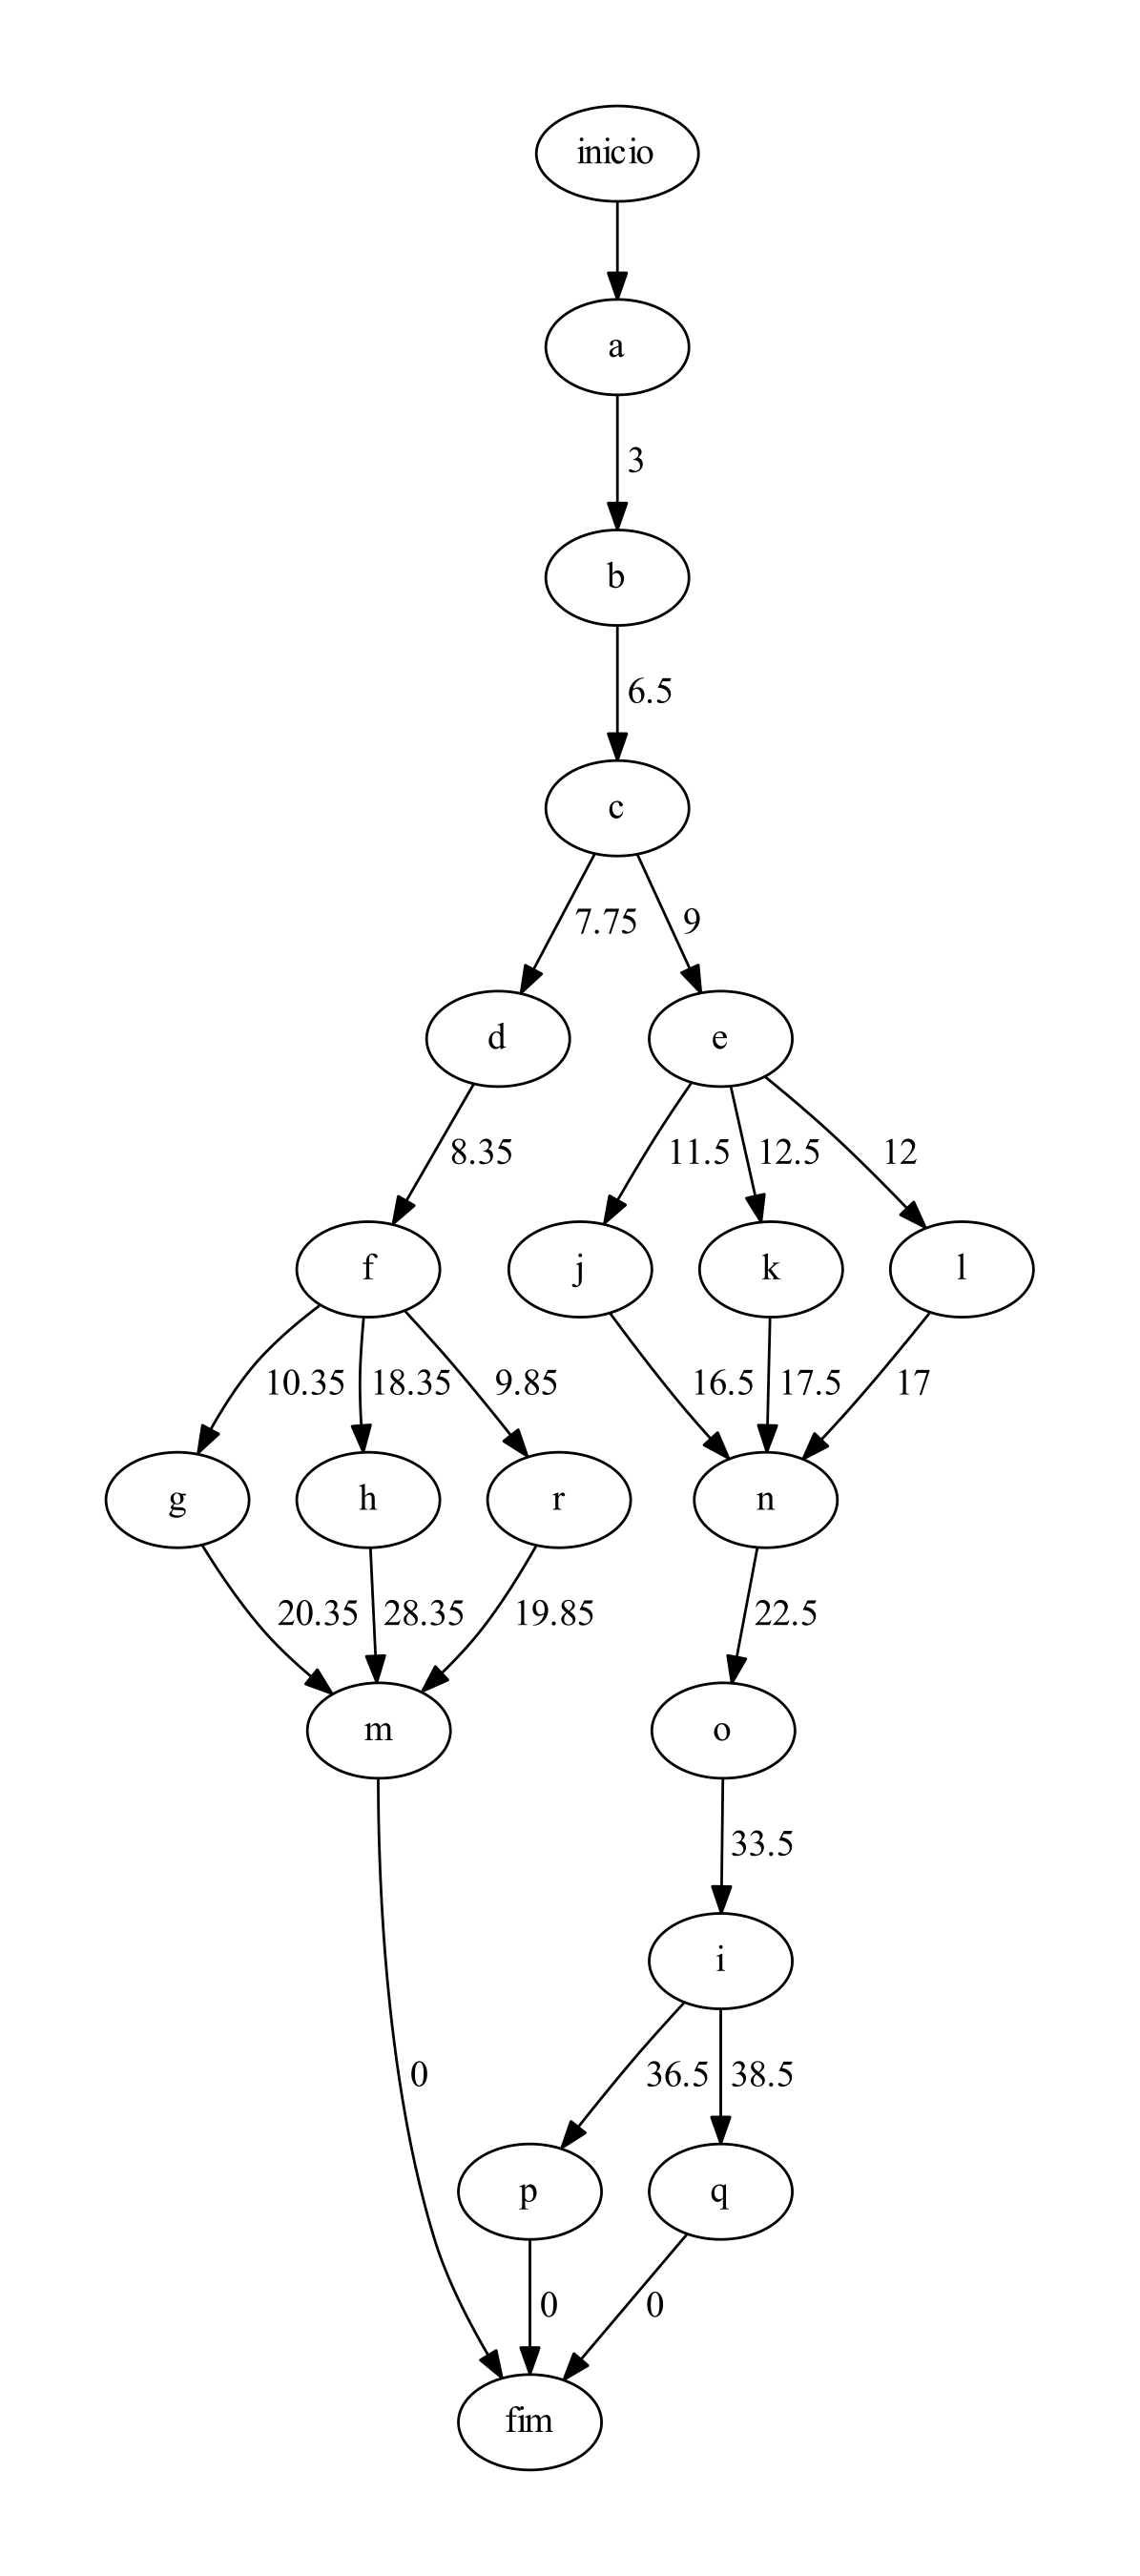
\includegraphics[scale=0.25]{CedoGraph1.png}
\caption{ Caminho Cedo}}
\end{figure}
\begin{figure}\centering{
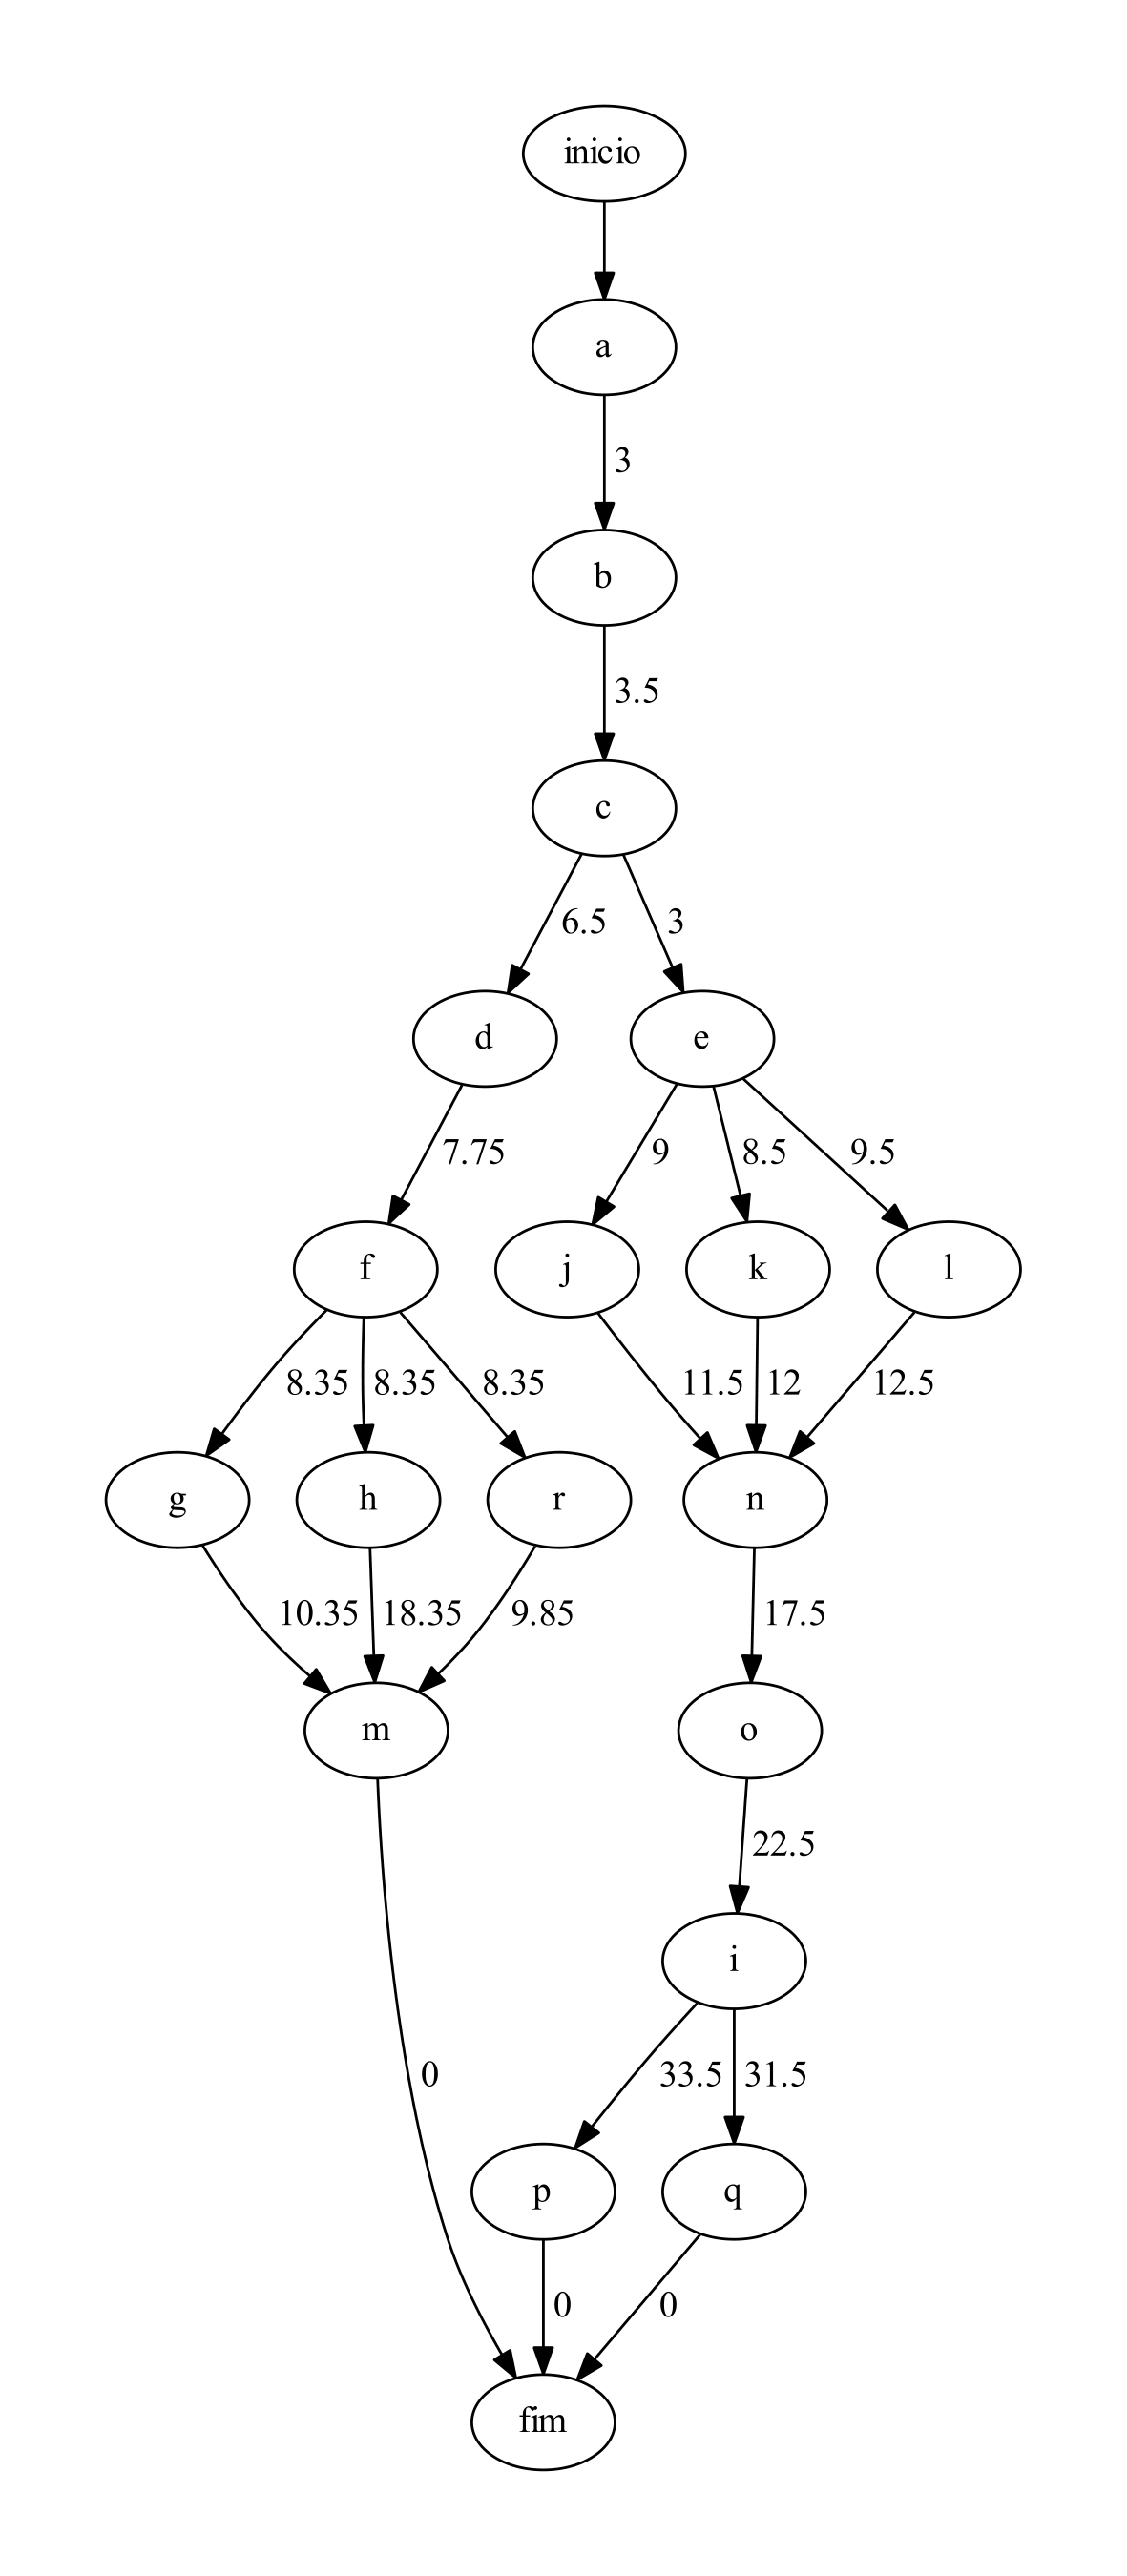
\includegraphics[scale=0.25]{TardeGraph1.png}
\caption{ Caminho Tarde}}
\end{figure}
\newpage
\section{Bibliografia}
http://www.workbreakdownstructure.com/\\
http://projetoseti.com.br/criar-a-estrutura-analitica-do-projeto-eap/\\
http://stakeholdernews.com.br/artigo/estimativas-tempo-e-custo-investimentos/\\
http://www.ime.usp.br/rvicente/PERT CPM

\end{document}
